%% $Id$
%%
%% Kapitel 2 - Die Oberflaeche
%%

\chapter{Benutzerinterface}

\section{"Uberblick}

Das Men"u {\bf Datei} enth"alt Funktionen zur Dateiverwaltung, wie
beispielsweise "offnen und Schliessen. Weiterhin kann unter {\bf
Zuletzt benutzt} schnell auf die aktuellsten Dateien zugegriffen
werden. Unter {\bf Bearbeiten} sind Editorfunktionen enthalten. Die
einzelnen Komponenten werden in Kapitel~\ref{Qelltexteditor}
und~\ref{Beweiswerkzeuge} genauer betrachtet. Mit {\bf
Einstellungen...} kann die Schriftart und Gr"o"se global f"ur alle
Editorkomponenten gesetzt werden. Weiterhin stellt man hier die
Einf"arbung von Schl"usselworten im
Quelltexteditor~\ref{Qelltexteditor} ein. Das Men"u {\bf Beweis}
enth"alt die einzelnen Beweiswerkzeuge und dient dazu zwischen dem
{\bf Beginner} und {\bf Fortgeschrittener} Modus zu wechseln. Diese
Modi beeintr"achtigen die bei den Beweisschritten zur Verf"ugung
stehenden Regeln.

\section {Quelltexteditor}
\label{Qelltexteditor} Jede ge"offnete Datei wird in einem Tab
angezeigt, der den Dateinamen angibt. Zwischen den Tabs kann mit
{\bf Strg + Bildhoch/Bildrunter} und {\bf Alt + Rechts/Links}
gewechselt werden.

Jeder Datei ist eine Sprache fest zugeordnet. M"ochte man einen
Ausdruck in einer anderen Sprache beweisen, so kann man hierf"ur
einen neuen Editor "offnen und der Ausdruck kopieren. Alternativ
kann auch die Dateiendung einer gespeicherten Datei ge"andert
werden. Ist ein eingegebener Ausdruck fehlerhaft, so wird dies links
von der betroffenen Zeile durch ein Error-Icon markiert. Zus"atzlich 
wird der fehlerhafte Teil rot unterstrichen.

Bewegt man den Mauszeiger "uber den markierten Text oder das Error-Icon,
so erscheint ein Tooltip, der den Fehler genauer beschreibt. Ein Klick
auf das Error-Icon bewirkt, dass fehlerhafte Text markiert wird. Wird
nun noch einmal auf das Error-Icon geklickt, wird der markierte Text
entfernt.

Der Quelltexteditor hebt freie Identifier und Type-Namen in der eingestellten
Farbe und fett hervor, da freie Identifier oder Type-Namen meist auf eine
fehlerhafte Eingabe zur"uckzuf"uhren sind. Gibt der Anwender zum Beispiel
\glqq{\bf let x = a in x}\grqq\ ein, ist dies nat"urlich nicht falsch, aber
der Type Checker w"urde den Ausdruck nicht akzeptieren, da das \glqq{\bf a}\grqq\ 
in der Expression frei vorkommend ist.

\subsection{Auto-Vervollst"andigung}
\label{Auto-Vervollstaendigung}
\index{Auto-Vervollst""andigung}
Der Quelltexteditor besitzt eine Auto-Vervollst"andigung. Gibt der Benutzer
den ersten Teil einer Expression ein, erscheint in der betroffenen Zeile ein
gelbes Dreieck mit einem Ausrufezeichen. Bewegt man den Mauszeiger "uber
das Icon, so erscheint ein Tooltip, der einen Vorschlag angibt, was der
Benutzer noch eingeben muss, um die Expression zu vervollst"andigen. Der
Tooltip gibt ebenfalls an, um welche Expression es sich handelt, was
besonders f"ur Unge"ubte eine wertvolle Information ist.

Die Expression die noch vervollst"andigt werden muss, wird im Hintergrund
hervorgehoben, so dass der Anwender genau erkennen kann, welchen Teil er
noch vervollst"andigen muss. Gibt der Anwender \glqq{\bf 1 + let x =}\grqq\ 
ein, wird der Teil \glqq{\bf let x =}\grqq\ hervorgehoben und der Tooltip
verr"at dem Anwender, dass er noch \glqq{\bf e1 in e2}\grqq\ eingeben muss
um \glqq{\bf Let}\grqq\ zu vervollst"andigen.

Der Anwender hat die M"oglichkeit auf das Icon zu klicken und der Vorschlag
wird automatisch an der richtigen Stelle eingef"ugt. Im gegebenen Beispiel
wird der Ausdruck \glqq{\bf 1 + let x =}\grqq\ automatisch zu
\glqq{\bf 1 + let x = e1 in e2}\grqq\ erweitert, was f"ur den Parser einen
g"ultigen Ausdruck darstellt. Die Auto-Vervollst"andigung ist ebenfalls in
der Lage Fehler innerhalb eines Ausdrucks zu erkennen und durch einen Klick
auf das Icon zu beheben.


\section {Outline}
\label{Beweiswerkzeuge}
\index{Outline}
TODO Christian







\section {Beweiswerkzeuge}
\label{Beweiswerkzeuge} Wird ein Beweiswerkzeug gestartet, so wird
es zus"atzlich zum Quelltexteditor im Tab der Datei angezeigt. F"ur
jede Datei kann jeweils nur ein Small Step Interpreter, ein Big Step
Interpreter und ein Type Checker aktiv sein. Diese k"onnen "uber die
entsprechende Schaltfl"achen angew"ahlt werden. Wird ein
Beweiswerkzeug erneut gestartet, so ersetzt der neue Beweis ein ggf.
schon aktives Beweiswerkzeug des selben Typs. M"ochte man also zum
Beispiel einen Small Step Beweis neu starten oder f"ur einen leicht
ge"anderten Ausdruck erneut ausf"uhren, so kann dies "uber eine
erneute Anwahl der Small Step Funktion im Men"u {\bf Beweis}
geschehen. Dabei wird jedoch der aktive Small Step Interpreter durch
den neuen ersetzt.

Jedes Beweiswerkzeug verf"ugt "uber einen {\bf Beginner} und einen
{\bf Fortgeschrittener} Modus. Diese Modi unterscheiden sich in den
Regeln, zum Beweis des Ausdrucks zur Verf"ugung stehen.

\section {Tutorials}
Im folgenden wird anhand von einigen Beispielen in die
Funktionsweise der einzelnen Beweiswerkzeuge eingef"uhrt. Zun"achst
"offnen wir "uber {\bf Datei} $\rightarrow$ {\bf Neu...} einen
Editor. Wie gesagt ist jeder Editor fest mit einer Sprache
verkn"upft.

\begin{figure}[h]
\begin{center}
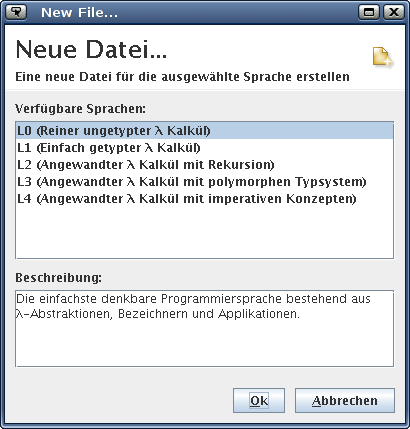
\includegraphics[width=7cm]{images/new-dialog.png}
\caption{Eine neue Datei erstellen}
\end{center}
\end{figure}

Wir w"ahlen f"ur unser Beispiel die Sprache \LONE\ aus und best"atigen
mit {\bf Ok}. Es ist nun standardm"a"sig der Quelltexteditor aktiv.
Wir geben einen Ausdruck ein, mit dem wir nun arbeiten wollen:

{\bf (lambda x.x * 3) 4}

Mit ein wenig Vorstellungskraft erkennt man, dass dieser Ausdruck
vorraussichtlich das Produkt aus 3 und 4 berechnet.


\subsection{Small Step Interpreter}
Unsere mutige Behauptung wollen wir nun nat"urlich durch einen
stichhaltigen Beweis untermauern. Wir starten also mittels {\bf
Beweis} $\rightarrow$ {\bf Small Step} oder mit der Taste F9 einen
Small Step Interpreter.

\begin{figure}[h]
\begin{center}
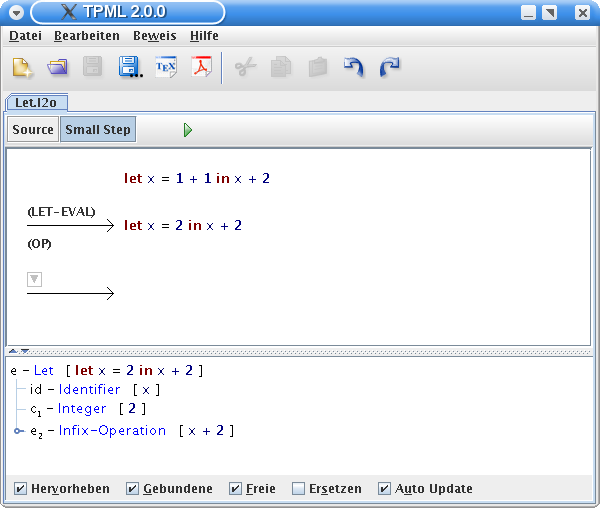
\includegraphics[width=7cm]{images/small-step.png}
\caption{Der Small Step Interpreter}
\label{FigureSmallStep}
\end{center}
\end{figure}

Bewegt man nun den Mauscursor "uber den Buttons des Regelmen"us
oberhalb des Pfeils f"ur den ersten Ableitungsschritt wird der Teil
des Ausdrucks rot unterstrichen, der als n"achstes Abgeleitet werden
soll, wie in Abbildung~\ref{FigureSmallStep} gezeigt.
In unserem Falle ist dies der gesamte Ausdruck. Der n"achste
Ableitungsschritt muss {\bf BETA-V} sein, um die 4 f"ur das x zu
substituieren. Wir klicken also auf den Button und w"ahlen in dem
erscheinenden Regelmen"u den entsprechenden Eintrag aus. Alternativ
kann man auch einzelne Schritte oder den kompletten Beweis
automatisch ausf"uhren lassen. F"ur einzelne Schritte klickt man
entweder auf den gr"unen Pfeil oberhalb des Small Step Interpreters
oder w"ahlt {\bf Raten} im Regelmen"u. Eine komplette Beweisf"uhrung
wird mittels {\bf Vervollst"andigen} im selben Men"u vorgenommen.

Ist man mit den Regeln vertraut, so kann man "uber {\bf Beweis}
$\rightarrow$ {\bf Fortgeschrittener} einige Regeln ausblenden. Das
Regelmen"u enth"alt nun nur noch Regeln die spezifizieren was getan
werden soll und nicht mehr genau wo. So muss zum Beispiel eine
Bedingung nicht mehr mit {\bf COND-EVAL} ausgewertet werden. Man
gibt w"ahlt lediglich {\bf COND-TRUE} bzw. {\bf COND-FALSE} aus.

\subsection{Big Step Interpreter}
Der Big Step Interpreter kann auch "uber das {\bf Beweis} Men"u oder
mit der Taste F11 gestartet werden. Zu beachten ist, dass man sich
hierf"ur nicht zwingend im Quelltexteditor befinden muss. Auch beim
Big Step Interpreter k"onnen Regeln "uber das Regelmen"u ausgew"ahlt
werden. Ist ein Unterbaum vollst"andig ausgewertet, so wird das
ermittelte Ergebnis f"ur h"ohere Knoten "ubernommen. Da unser
Beispiel lediglich einen Unterbaum f"ur die Regel {\bf BETA-VALUE}
enth"alt, ist dies auch gleichzeitig unser Ergebnis. Im Gegensatz
zum Small Step Interpreter gibt es aufgrund der Baumstruktur des
Beweises mehrere Stellen an denen Regeln angewandt werden k"onnen.
Die Raten-Funktion bezieht sich dabei immer auf den obersten, noch
nicht komplett ausgewerteten Teilbaum. Mit {\bf Vervollst"andigen}
wird stets nur der jeweilige Unterbaum komplett ausgewertet und
nicht wie beim Small Step Interpreter der komplette Beweis zu ende
gef"uhrt.

\subsection{Type Checker}

Diese Beweisart ist genau wie der Big Step Interpreter in einer
Baumstruktur aufgebaut. Der Type Checker verh"alt sich daher
bez"uglich des Anwenden von Regeln, den Raten und der
Vervollst"andigen Funktion genau wie der Big Step Interpreter. Das
Anf"ugen von Typvariablen geschieht bei Regelanwendung automatisch.

Alternativ kann man mit der Funktion {\bf Typ eingeben} in dem
Regelmen"u selbst einen Typ f"ur den entsprechenden Teilbaum
eingeben, wie in Abbildung~\ref{FigureTypeChecker} gezeigt.
Der Typinferenzalgorithmus versucht dann den Unterbaum zu
diesem Typ auszuwerten.

\begin{figure}[h]
\begin{center}
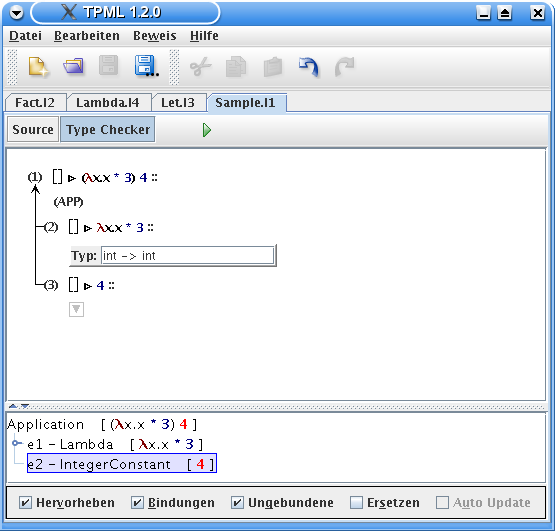
\includegraphics[width=7cm]{images/type-checker.png}
\caption{Der Type Checker}
\label{FigureTypeChecker}
\end{center}
\end{figure}

\subsection{Type Inference}
Der Type Inference Algorithmus ist, wie der Small Step Interpreter 
auch, in einer Listenstruktur realisiert, und kann "uber {\bf Beweis} 
$\rightarrow$ {\bf Type Inference} gestartet werden. Die Bedienung ist auch diesmal 
wieder an die bereits genannten Beweisarten angelehnt. Es besteht 
auch hier die M"oglichkeit selber Regeln auf den aktuellen Ausdruck
anzuwenden, den n"achsten Schritt erraten zu lassen, oder den kompletten
Ausdruck zu vervollst"andigen.

Wendet man die Regel Unify an, werden die evtl. daraus hervorgehenden
Type Substitutions in einer Liste "uber den Type Formulas gesammelt. 
Dabei ist die zuletzt gesammelte Type Substitution sichtbar. Die bereits
vorher gesammelten Type Substitutions werden durch drei Punkte angedeutet,
und k"onnen als Tooltip "uber den Punkten eingesehen werden.

Wenn man sich etwas mit der Funktionsweise des Algorithmus vertraut gemacht hat,
kann man "uber {\bf Beweis} $\rightarrow$ {\bf Fortgeschrittener} in den 
Advanced Modus wechseln. In diesem Modus werden Type Equations, bei denen beide
Typvariablen aus Arrow Types bestehen, jetzt nicht mehr neue Type Equations
aufgenommen, sondern diese werden direkt zu Type Substitutions aufgel"ost.
Ausserdem wird beim Anwenden einer Regel auf den Ausdruck nicht mehr vom System
versucht die Regel einer Type Formula zuzuordnen, sondern es wird versucht die Regel
auf die erste Type Formula anzuwenden. Diese k"onnen allerdings durch Drag 
and Drop umsortiert werden.

Das Regelwerk ist, mit einer Ausnahme, "aquivalent zum Type Checker. Es wurde 
noch die Regel {\bf UNIFY} hinzugenommen. Die sich aus folgenden Ableitungsschritten
zusammensetzt:\\[4mm] 

\begin{tabular}{ll}
  (EMPTY)\    & $\unify(A,\emp) = [\,]$ \\[3mm]
  (ASSUME)\   & $\unify(A,\{\tau = \tau'\} \cup E) = \unify(A,E) \mbox{  falls } (\tau = \tau') \in A $\\[3mm]
  (TRIV)\     & $\unify(A,\{\tau = \tau\} \cup E) = \unify(A,E)$\\[3mm]
  (MU-LEFT)\  & $\unify(A,\{\rectype{t}{\tau} = \tau'\} \cup E) = 
                 \unify(A,\{\tau [\rectype{t}{\tau}/t] = \tau'\} \cup E)$\\[3mm]
  (MU-RIGHT)\ & $\unify(A,\{\tau = \rectype{t}{\tau'}\} \cup E) = 
                 \unify(A,\{\tau = \tau' [\rectype{t}{\tau'}/t]\} \cup E)$\\[3mm]
  (VAR)\      & $\unify(A,\{\alpha = \tau\} \cup E) = \unify(A,\{\tau = \alpha\} \cup E)$\\[2mm]
              & $\ =\, \bcase 
                        [\tau/\alpha] \circ s & 
                        \mbox{falls } \alpha \notin \var{\tau} \mbox{ und } 
                        \unify(E[\tau/\alpha]) = s \\[2mm]
                        \fail         & \mbox{falls } \alpha \notin \var{\tau} \mbox{ und }\\&
                        \unify(E[\tau/\alpha]) = \fail\\[1mm]
                        & \mbox{oder } \alpha \in \var{\tau} \mbox{ und } \alpha \neq \tau
                        \ecase\vspace{3mm}$\\
  (ARROW)\    & $\unify(A,\{\tau_1 \to \tau_2 = \tau'_1 \to \tau'_2\} \cup E)$\\[1mm]
              & \quad $= \unify(A \cup \{\tau_1 \to \tau_2 = \tau'_1 \to \tau'_2\},
                \{\tau_1 = \tau'_1,\,\tau_2 = \tau'_2\} \cup E)$\\[3mm]
  (TUPLE)\    & $\unify(A,\{\tau_1 *\ \ldots\ * \tau_n = \tau_1' *\ \ldots\ * \tau_n'\} \cup E)$\\[1mm]
              & \quad $= \unify(A \cup \{\tau_1 *\ \ldots\ * \tau_n = \tau_1' *\ \ldots\ * \tau_n'\},$\\
              & \quad \quad $\{\tau_1 = \tau_1',\ \ldots\ , \tau_n = \tau_n'\} \cup E)$\\[3mm]
  (LIST)\     & $\unify(A,\{\listtype{\tau} = \listtype{\tau'} \} \cup E)$\\[1mm]
              & \quad $= \unify(A \cup \{\listtype{\tau} = \listtype{\tau'} \},
                         \{\tau = \tau' \} \cup E)$\\[3mm]
  (REF)\      & $\unify(A,\{\reftype{\tau} = \reftype{\tau'} \} \cup E)$\\[1mm]
              & \quad $= \unify(A \cup \{\reftype{\tau} = \reftype{\tau'} \},
                         \{\tau = \tau' \} \cup E)$\\[3mm]
  (OBJECT)\   & $\unify(A,\{\objecttype{\phi}\ =\ \objecttype{\phi'} \} \cup E)$\\[1mm]
              & \quad $= \unify(A \cup \{\objecttype{\phi}\ =\ \objecttype{\phi'} \},
                         \{\phi = \phi' \} \cup E)$\\[3mm]
  (ROW)\      & $\unify(A,\{ (m_1 = \tau_1\ ;\ \ldots\ ;\ m_n = \tau_n;\ \phi)$\\
              & \quad $= (m_1 = \tau_1'\ ;\ \ldots\ ;\ m_n = \tau_n';\ \phi') \} \cup E)$\\[1mm]
              & \quad $= \unify(A \cup \{ (m_1 = \tau_1\ ;\ \ldots\ ;\ m_n = \tau_n;\ \phi)$\\
              & \quad \quad $= (m_1 = \tau_1'\ ;\ \ldots\ ;\ m_n = \tau_n';\ \phi') \},$\\
              & \quad \quad \quad $\{\tau_1 = \tau_1', \ \ldots\ ,\tau_n = \tau_n',
                \phi = \phi' \} \cup E)$\\[3mm]
  (STRUCT)\   & $\unify(A,\{\tau_1 = \tau_2\} \cup E) = \fail$\\[1mm]
              & in  allen anderen F\"allen
\end{tabular}\\[6mm]
Bei der Regel {\bf ROW} ist darauf zu achten, dass die Methodennamen nicht in der gleichen Reihenfolge
vorkommen m"ussen. Ebenfalls m"ussen die Methodennamen nicht in beiden Reihen vorkommen, da f"ur den Fall, 
dass $\phi$ nicht gleich $\epsilon$ ist, $\unify$ auch mit $\phi$ und den restlichen Methoden von $\tau'$ 
aufgerufen werden kann. Zum Beispiel f"uhrt $\unify (A,\{ (b: \alpha_1 ; \alpha_2) = (a: int ; b: int ;)\}
\cup E)$ zu dem Aufruf von $\unify (A \cup \{ (b: \alpha_1 ; \alpha_2) = (a: int ; b: int ;)\},
\{\alpha_1 = int, \alpha_2 = a: int\} \cup E)$.


% vi:set syntax=tex ts=2 sw=2 et encoding=UTF-8:
